% Use class option [extendedabs] to prepare the 1-page extended abstract.
\documentclass[extendedabs]{bmvc2k}

% For the final submission, comment out the bmvcreviewcopy so that
% author names etc appear.
%\bmvcreviewcopy{1234}

% Enter a shortened version of the title as a running header.
% For two authors, enter both surnames, separated by commas.  For
% more than two authors, the first author's name followed by
% \bmvaEtAl will produce the correct output (uppercase author name,
% lowercase etal).  This will not appear in the extended abstract
\runninghead{Claus, Fitzgibbon}{Plumbline Constraint for the RF Model}
% \runninghead{Claus \bmvaEtAl}{Plumbline Constraint for the RF Model}

% Document starts here
\begin{document}

\title{Pedestrian Analysis}

% Notice that there is a reasonable amount of whitespace around the
% author names.  There should be no reason to compress this for the
% online proceedings as the page limit is counted from the bottom
% of the author list.
%
% While it may be tempting to compress this for the extended
% abstract, please resist the temptation to overdo it.  This 1-page
% abstract is currently three pages in normal BMVC style, which
% should be plenty of space for your key idea, figure, and
% references.
\addauthor{Ashish Kumar}{2016CSB1033}{1}

\addinstitution{
Department of Computer Science,\\
 IIT Ropar}
 
 \addauthor{Chirag Khurana}{2016CSB1037}{2}

\addinstitution{
Department of Computer Science,\\
 IIT Ropar}
\maketitle

% Extended abstract begins here.  In a one-page document, there is
% little need for section headers, but you may use \section etc if you
% wish.

\section{Abstract}
In systems like self driving cars and diving assistants, protection of pedestrians is the most important component to be taken care of. The system needs to be able to tell which direction the pedestrian is walking and whether the pedestrian is distracted or not. With the recent advancements in deep learning, it has become possible to do this task with high accuracy. We propose a deep learning based solution for this problem which uses transfer learning and knowledge distillation \cite{hinton2015distilling}.

\section{Introduction}
There are many incidents involving vehicles where the safety of pedestrians is at risk. If a system is there which can predict the direction in which the pedestrian will be moving, it can help avoid many accidents. Also, with the recent advancements in technology and hardware, self driving cars have been made possible. The self driving cars also need a system to provide safety to the pedestrians. A system is required which can be helpful in pedestrian safety. The system should be able to predict the direction of motion of pedestrian so that further actions can be taken accordingly. Also, the system also needs to be able to detect whether the pedestrian is distracted or not. If the pedestrian is distracted, then even if the pedestrian is not moving in a trajectory towards the vehicle, proper precautions have to be taken. \\
In the subsequent sections, we address the problem of pedestrian direction and distraction prediction. 

\section{Related Work}
\subsection{Direction Estimation of pedestrian from multiple still images}
This is a review of paper \cite{1336451}.
The idea of this paper is very simple. Haar wavelet coefficients (8x8 pixels) are used to generate
feature vectors for each image. They are using three different orientations of Haar wavelet (horizontal, vertical and diagonal). These are used to represent the feature vector for an image.
\newline 
The problem is treated as a classification problem. SVM classifiers for 16 directions (i.e, 0, 22.5, 45, ... 337.5) are trained using the Haar features extracted earlier. During inference, class which gets the maximum score on SVM output is the prediction.
\newline
Scores are calculated by taking weighted sum of target class and its neighbour class. For example, if we
are to compute the score for direction 45, the the score with weight w will be:
\begin{equation}
Score = w*s_{45} + ( s_{22.5} + s_{67.5} )
\end{equation}

\subsection{Image Based Estimation of Pedestrian Orientation for Improving Path
Prediction}
This is a review of paper \cite{4621257}. In this paper, they have tried to do pedestrian walking direction prediction both using just a single
image and sequence of image.

\subsubsection{Single image}
First, bounding box is made for a detected person. After that gradient directions are calculated for each pixel. Then, the image is subdivided into MxN blocks and gradient direction is quantized into K bins each spanning 360/K degrees. For each bin ${(m, n, k)}$, number for pixels are counted in the block (m, n) having gradient direction in bin k. This way, an MxNxK feature vector is formed. 
\newline 
Once this has been done, an SVM is trained for each of the K bins, and maximum score is used to get the direction prediction.

\subsubsection{Sequence of images}
In order to improve the reliability of classification, the single frame classification probabilities computed above are integrated in a Bayesian framework of a Hidden Markov Model (HMM) \cite{rabiner1989tutorial}. The evolution of pedestrian orientation over time is modeled as a Markov chain governed by transition probabilities between different orientation states. The transition probabilities between orientation classes over a single time step are given by the matrix of values in ${P(c_t \mid c_{t-1})}$. The class conditional probabilities ${P(o_t\mid c_t)}$ are proportional to the posterior probabilities P(ct|ot) of the classes given by the SVM classifier. At each time step ${t}$, the class probabilities estimated by integrating t image frames are computed recursively from those from ${t-}$1 frames using the equations: 
\newline
Prediction Step:
\begin{equation}
P(c_t \mid o{1:t-1}) = \sum c_tP(c_{t-1} \mid c_{t-1})P(c_{t-1} \mid o_{1:t-1})
\end{equation}
Correction Step:
\begin{equation}
P(c_t \mid o_{1:t}) = \frac{P(o_t \mid c_t)P(c_t \mid o_{1:t-1})}{\sum_{ct} P(o_t \mid c_t)P(c_t \mid o_{1:t-1})}
\end{equation}
The prediction step smoothens the probability estimates obtained from previous observations whereas the observation step weights the probabilities according to the current observation. For predicting the future orientation probabilities, the prediction equation is applied repeatedly over a number of time steps without performing the observation step. The transition probabilities can be learned based on observing state transitions in a given sequence of pedestrians.
\newline

${P(c_t \mid c_{t-1})}$ = ${\frac{\text{\# transition with orientation change}}{\text{\# Total time steps}}}$

\subsection{Estimation of Pedestrian Walking Direction from Video}
This is a review of paper \cite{8259689}. It is assumed that the pedestrian is walking following a given direction. The image sequence is acquired and segmented. The problem of direction change is not processed here. The direction is predicted using principal point $u_o$ and focal length f of the camera. Let $\omega(u_{\omega},v_{\omega})$ be the vanishing point located on the image plane associated to the direction of $\Delta^{'}$, vanishing point is the point of intersection of the line joining the top and line joining the bottom of the detected pedestrian body in the sequence of images. The angle $\alpha$ may be computed using $\omega$, the focal length f and the coordinates of the principal point $P(u_{o},v_{o})$ as follow:
\begin{equation}
    \alpha = arctan(\frac{u_{\omega}-u_{o}}{f})
\end{equation}
And f and $u_{o}$ are computed using some known sequence of images and their direction as folows:
\begin{equation}
    f = \frac{u_{\omega1}-u_{\omega2}}{tan(\alpha1)-tan(\alpha2)}
\end{equation}
But this algorithm is very limited. It may fail if ground level is non-planar, if images are taken from the top view, if the head of the pedestrian is inclined, if the camera is moving, if the pedestrian is walking parallel or perpendicular to the camera, etc.


\section{Methodology}
We used the following method to develop a robust pipeline for pedestrian direction and distraction prediction.

\subsection{Dataset Collection}
No proper dataset could be found on the internet for this problem. Using arbitrary images or videos from the internet was not possible since that would increase the difficulty in labelling the dataset. Therefore we created our own dataset containing a total of 3105 images. We collected videos of different people with different backgrounds. The collected videos were converted to images at a rate of 1 out of 5 frames. Even then, we found that many images consisted of the person standing in the same pose with the same background, therefore, in the interest of memory and training time, we removed such images as they provided no new relevant information. All images are divided into the following 8 bins each of size 45: 0, 45, 90, 135, 180, 225, 270, and 315 according to the nearest angle of walking direction. For example, if the person is moving away from the camera, then the angle is 0, if the person is going straight towards right, then the angle is 90, and so on. All images are also labelled with either 1 or 2, 1 for concentrated and 2 for distracted person during walking. Person detection has been done on the images thus obtained using Single Shot Multibox Detector \cite{liu2016ssd} with MobileNet \cite{howard2017mobilenets} as backend.

\subsection{Preprocessing data}
For preprocessing, the images were first resized to 128x128. After that, the iamges were preprocessed according to the MobileNet standard, i.e, 128 was subtracted from each pixel and then each pixel was divided by 128 in an image.

\subsection{Non Deep Learning Approach}
\begin{figure}[t]
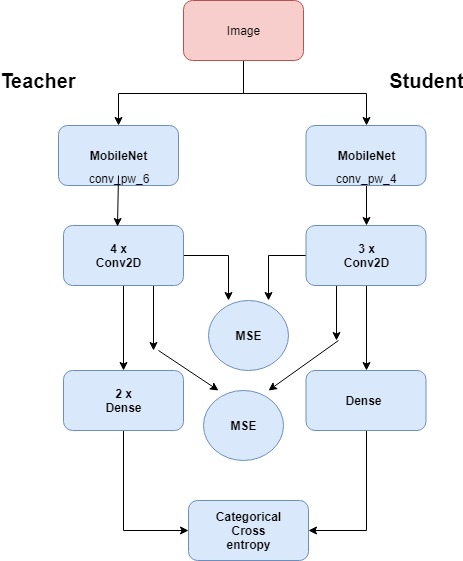
\includegraphics[width=\linewidth]{images/KD.jpg}
\caption{
Student and teacher model for knowledge distillation.}
\label{fig:KD}
\vspace{-2mm}
\end{figure}
\subsubsection{Baseline Approach}
Since all the previous research that has been done in the field was based on conventional computer vision algorithms, we tried to solve the problem using conventional computer vision algorithms. Since we need features from the image in order to perform any classification, we used the Histogram of Oriented gradients \cite{dalal2005histograms} as our feature extractor. The HOG features of each image are of 3780 dimensions. After that, we use a Support Vector Machine classifier \cite{hearst1998support} which uses the HOG feature of the image as input and the direction angles as output labels.

\subsubsection{Enhanced Approach}
Using HOG as feature extraction only provides the global features in an image but in this problem, local features can also be very useful in the classification task. We tried to use sift features as local features but the sift algorithm could not find interest points that can be useful for direction prediction of pedestrians. Therefore, we used pyramid of histogram of Gaussian to get some level of local features. We used 4 layers of pyramid and used the HOG features extracted from these layers as input to the SVM.

\subsection{Deep Learning Approach}
Deep learning has proven remarkable in many computer vision based problems. We prepared two different types of models for prediction using deep learning. The first one is for low end devices and requires very less computational power, but it only deals with the prediction of pedestrian direction. The second model requires more computational power and deal with both direction prediction and distraction prediction.

\begin{figure}[t]
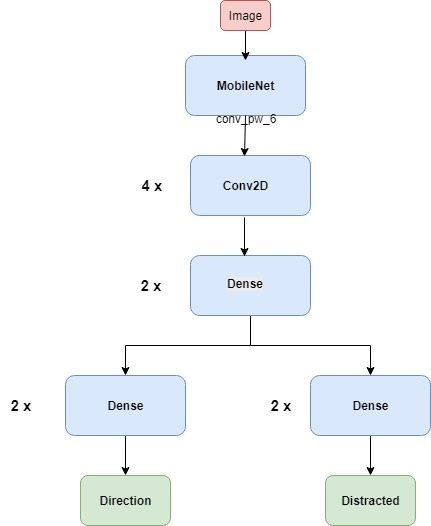
\includegraphics[width=\linewidth]{images/Full.jpg}
\caption{
High computation model for direction and distraction prediction.}
\label{fig:FULL}
\vspace{-2mm}
\end{figure}


\subsubsection{Low Computational Model}
We first trained a large model to predict the walking direction of pedestrians. The input to the model was image of dimension 128x128. The model consisted of a pre-trained MobileNet model with layers till 'conv\_pw\_6' layer of MobileNet model. After this, a few convolutional and fully connected layers were added. The whole model was trained on the training data (all the layers of MobileNet were set trainable). This model achieved a validation accuracy of 96.13\% and a training accuracy of 99.12\%. Since this model was large, we created another smaller model with fewer layers, and used the concept of knowledge distillation \cite{hinton2015distilling}. The intuition behind knowledge distillation is that we are trying to make a student model mimic the teacher model by using the softmax output of the teacher model to train the student model. We used the large model as the teacher model and the small model as the student model. The small model had MobileNet layers till 'conv\_pw\_4' and a few convolutional and fully connected layers after that. Temperature for knowledge distillation was set to be 7 which was chosen after repetitive experimentation.
\\
Using just this, we were unable to get any statistically important gain in accuracy, therefore, we extended the concept of knowledge distillation. Instead of using just the last softmax layer of large model for knowledge distillation, we added a few more layers for knowledge distillation. We used 2 convolutional layers in large model which had a corresponding layer in small model (i.e layers in small model which have the same input and output dimensions as these layers) and we distilled the knowledge from these convolutional layers of large model to the convolutional layer in small model. The intuition behind this extension is that, since we are trying to make the smaller model mimic the larger model, we can provide the smaller model some extra help by making the values of intermediate layers of smaller model similar to the intermediate layers of the larger model. Using this, we noticed a gain of 3\% in validation accuracy. Without any knowledge distillation, the accuracy of the small model on validation set was 89.1\%, using knowledge distillation only on output layer resulted in a validation accuracy of 90.9\%, using knowledge distillation on the output layer and internal convolutional layers resulted in a validation accuracy of 94.3\%. The setup for training the low computational model is shown in figure \ref{fig:KD}. We tried to do knowledge distillation for both distraction and direction prediction also, but a common model for them with knowledge distillation is not able to perform well.

\begin{figure}[t]
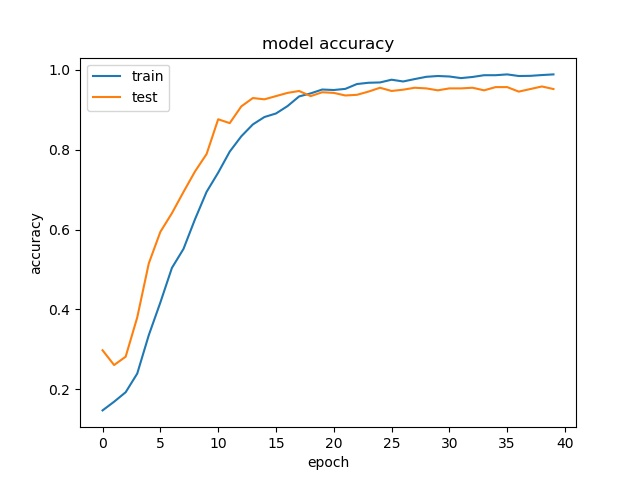
\includegraphics[width=\linewidth]{images/accuracy_teacher.jpg}
\caption{
Training and validation accuracy of teacher model.}
\label{fig:accteacher}
\vspace{-2mm}
\end{figure}

\begin{figure}[t]
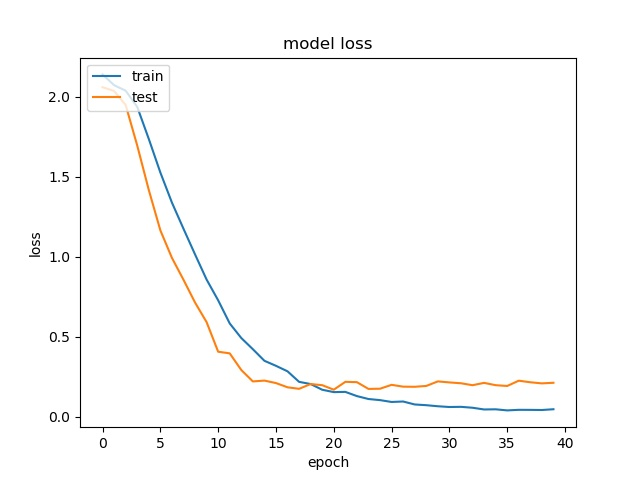
\includegraphics[width=\linewidth]{images/loss_teacher.jpg}
\caption{
Training and validation loss of teacher model.}
\label{fig:lossteacher}
\vspace{-2mm}
\end{figure}

\begin{figure}[t]
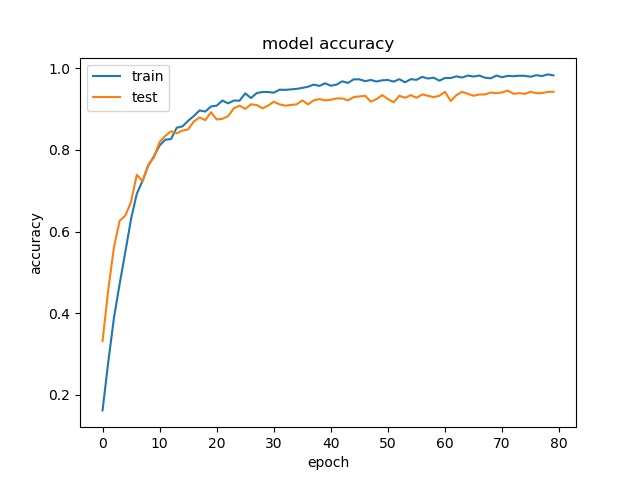
\includegraphics[width=\linewidth]{images/accuracy_student.jpg}
\caption{
Training and validation accuracy of student model.}
\label{fig:accstudent}
\vspace{-2mm}
\end{figure}

\begin{figure}[t]
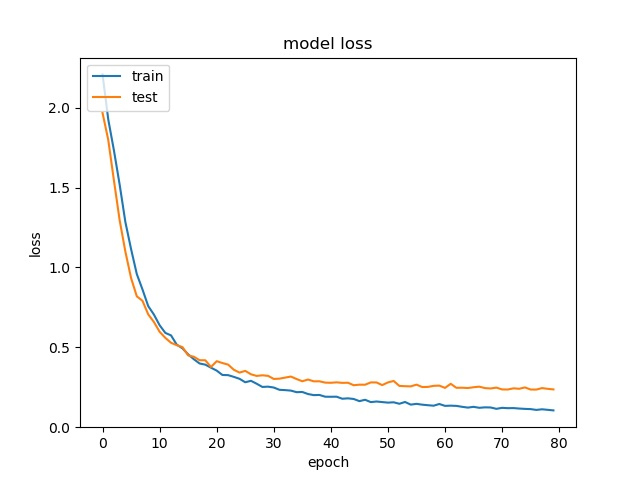
\includegraphics[width=\linewidth]{images/loss_student.jpg}
\caption{
Training and validation loss of student model.}
\label{fig:lossstudent}
\vspace{-2mm}
\end{figure}

\subsubsection{High Computation and accuracy model}
we used a large model which uses somepart of MobileNet as a hight computation model in order to get good validation accuracy. The model initally has some pretrained layers of MobileNet, then a few convolutional layers and then, the model is splits so that two outputs can be produced. One output is for direction prediction and the other is for distraction prediction. The setup for this model is shown in figure \ref{fig:FULL}

\section{Experimental Settings}
There are no particular experimental configurations in non deep learning techniques for completing this task. Here we discuss the experimental setup for deep learning based approach.



\subsection{Low computation model}
For the low computational model, the teacher network was trained with a learning rate of 0.00005. Adam optimization \cite{kingma2014adam} was used. The loss function used was categorical crossentropy loss. The learning rate for student model was 0.00005, Adam optimizer was used. The loss function for softmax output was categorical crossentropy and the loss function for error in the corresponding convolutional layers in teacher and student model was mean squared error. The temperature used for generating soft targets for knowledge distillation was 7.

\subsection{High computation model}
For the high computation model, learning rate used was 0.00005. Categorical crossentropy was used as loss function for direction prediction and binary crossentropy was used as loss function for distraction prediction.

\section{Results and Discussion}
Following is the detailed analysis of the results that we observed.

\subsection{Non Deep learning Algorithms}
\subsubsection{Baseline Model}
The baseline model consisted of HOG as feature representation and SVM for classification. With this pipeline, we were able to achieve a validation accuracy of 78.1\% with using 80\% data for training and 20\% for validation.

\subsubsection{Enhanced Model}
The enhanced model used HOG at different layers in a gaussian pyramid. This was done in order to include some contribution of local features in prediction. With the enhanced model, we achieved an accuracy gain of 2\%, the final validation accuracy using the enhanced model was 82\%. As expected, including local features did improve the classification accuracy although the gain is not statistically much important.

\subsection{Deep learning Algorithms}
\subsubsection{Low computational model}
The graph for accuracy and loss for training the teacher model are shown in figure \ref{fig:accteacher} and figure \ref{fig:lossteacher} respectively. \textbf{Please not that in the graph, initially validation accuracy is higher than training accuracy and validation loss is lower than training loss because of dropouts. We used Keras \cite{chollet2015keras} for our implementation, in keras, during training, inverse dropout is active which results in a lower accuracy, while when computing the validation accuracy, keras turns off the dropouts, and therefore the complete model is used. This results in higher accuracy for validation. In simple words, we can say that this is because when calculation training accuracy, the complete model is not used since dropout is active and hence that accuracy is not the accuracy of the whole model. If dropout had been off for calculating training accuracy, then the training accuracy would certainly be higher than validation accuracy.} The highest accuracy achieved for the teacher model was 95.81\%. The graph for accuracy and loss for training the student model using the teacher model is shown in figure \ref{fig:accstudent} and figure \ref{fig:lossstudent} respectively. The highest accuracy achieved using knowledge distillation was 94.3\%. Without using any knowledge distillation, the smaller model could only achieve a validation accuracy of 89.1\%.\\\\
Using knowledge distillation with the extension improved the validation accuracy remarkably. We only got a decrease of 1.51\% in validation accuracy and the model was compressed to almost a third. The size of the teacher model was 72 MB and the size of student model was 23 MB. The inference time also decrease by a huge margin. When used on a mobile phone, the teacher model had an inference time of 410 ms on an average and the student model had an inference time of 130 ms on an average.

\subsubsection{High Computation model}
The main reason we used high computational model was so that we could get good performance for both direction prediction and distraction prediction using a single model. This model was able to achieve a validation accuracy of 94.3\% for direction prediction. But, the validation accuracy for distraction prediction did not exceed 77.64\%. This was an expected observation because of two reasons:
\begin{itemize}
    \item Prediction of distraction is a very hard task. For person moving in different direction, the head movement angle for distraction has to be different and its very hard to tell what the person is distracted or not even for a human.
    \item Due to time limitations, the dataset prepared was not good enough for distraction prediction. There may have been some inconsistencies in the direction prediction dataset which led to such results.
\end{itemize}

\section{Summary and Future Work}
Safety off pedestrians on road is one of the most important and highly researched areas in computer vision. In this report, we hav proposed a novel method based on neural network to predict the moving direction of pedestrian and estimate whether the pedestrian is distracted or not. Both the pedestrian moving direction and distraction results can be used for further decision making by automatic or semi-automatic vehicles to prevent mishappenings on roads.\\\\
In the approach we described in this report, we have only used the information present in one image. Temporal information can also be very useful in providing information for the prediction model, especially in case of distraction prediction. We believe that using temporal information can result in magnitudes of increase in prediction accuracy.

\section{References}
\bibliography{egbib.bib}

\end{document}


